\section{Dual-Piezo Setup}
\subsubsection*{Scan-Settings}
$f = 6.0$ Hz,  \\
Amplitude: 5.2 V,  \\
Offset: 0 V.  \\
Filename: \texttt{ALL0010.CSV}.   \\
Piezo No.; \texttt{2}  \\
Script: \texttt{plotPdPiezo.m} \\

I now tried to use both piezos simultaneously. One piezo was used to scan the cavity length, the other was used to moved the peaks relative to the cavity scan.
To do this, a DC voltage was applied to the second piezo. This lead to a constant offset between the two mirrors, thus moving the peaks around whilst not interfering with the cavity scan.

This also allowed us to get a better feeling for the behaviour of the cavity. 
We therefore assume, that the prior analysis of a 2000 finesse is \textbf{incorrect}.
We coupled light to the cavity such that there are now two prominent peaks.
Startin off with no offset, we get the following:


\begin{figure}[H]
    \centering
    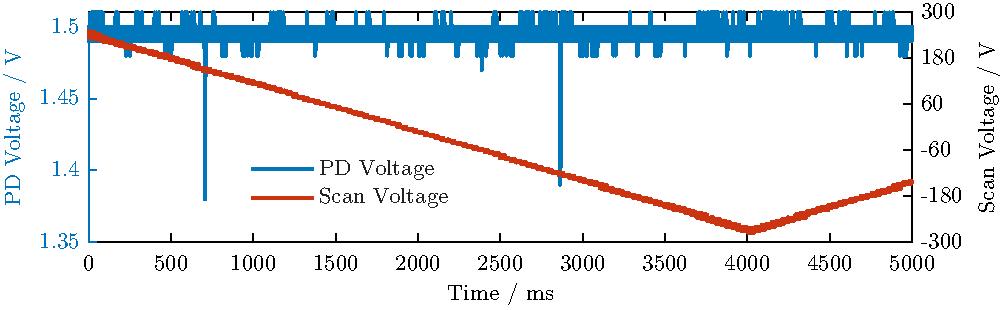
\includegraphics[width=\textwidth]{twoPiezo/Figure_1.pdf}
    \caption{The offset in this case was 0V.}
\end{figure}



\begin{figure}[H]
    \centering
    \begin{subfigure}[t]{0.48\textwidth}
        \centering
        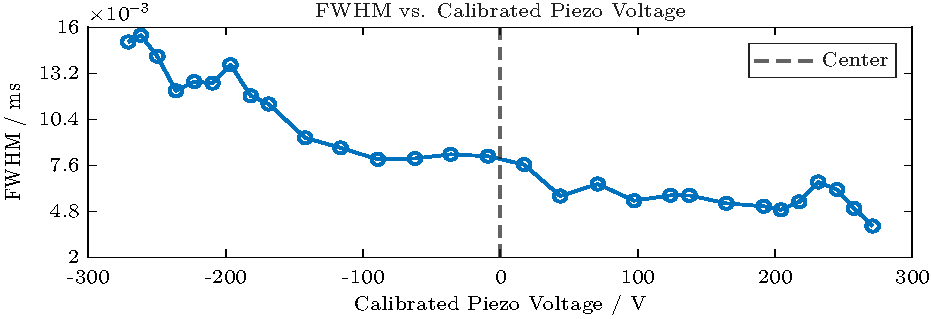
\includegraphics[width=\textwidth]{twoPiezo/Figure_3.pdf}
        \caption{Zoomed-in view of Peak 1.}
        \label{fig:peak1_0v}
    \end{subfigure}
    \hfill
    \begin{subfigure}[t]{0.48\textwidth}
        \centering
        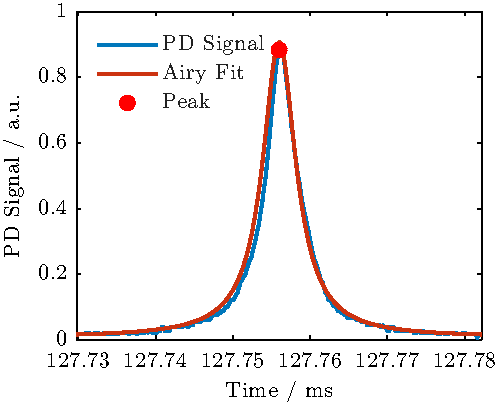
\includegraphics[width=\textwidth]{twoPiezo/Figure_4.pdf}
        \caption{Zoomed-in view of Peak 2.}
        \label{fig:peak2_0v}
    \end{subfigure}
    \caption{Zoomed-in views of the detected large peaks of one scan. The left one is cleary fuzzy and spread out.}
\end{figure}
This data corresponds to a finesse of $\mathcal{F}\approx11\,000$ - \textbf{much higher} than the previous value!
\newpage
\subsection{Offset 306V - Different FSR}
I tried to offset the peaks using the piezo (at 306 V) to see to different peaks in order to increase the quality of the left peak. 
However, this did not work.
When moving the right peak (here: peak 2 in Fig. \ref{fig:peak2_0v}) to the left of the frame (where currently peak 1 (Fig. \ref{fig:peak1_0v}) sits), it then gets fuzzy. 
So this means that the peak itself is not the issue, but perhaps the scan is not reliable in this region. This will later be analyzed.

It was however possible to see a new peak coming in from the right.
This is a good sign! 
This peak was of a good "qualitiy". In genereal, changing the offset of the second piezo did \textbf{not} change the signal much, but it made it possible to move the peaks around.


\begin{figure}[H]
    \centering
    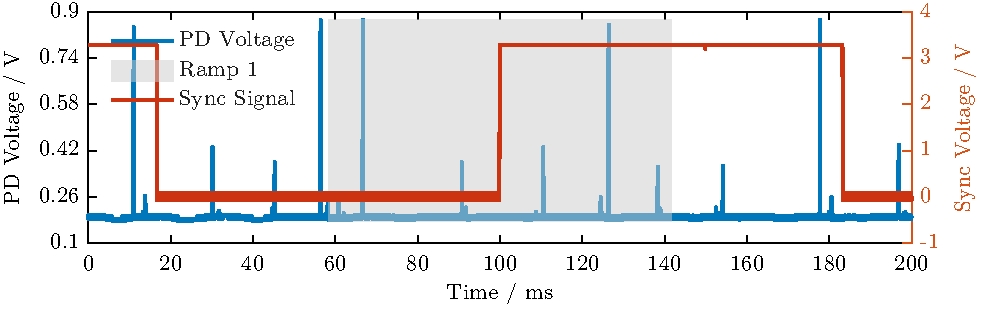
\includegraphics[width=\textwidth]{twoPiezo/Figure_11.pdf}
    \caption{Using the second piezo to move around the peaks, it was possible to see a new peak of similar and large amplitude. The offset in this case was 306V. File used: \texttt{ALL0015.CSV}}
\end{figure}


\begin{figure}[H]
    \centering
    \begin{subfigure}[t]{0.48\textwidth}
        \centering
        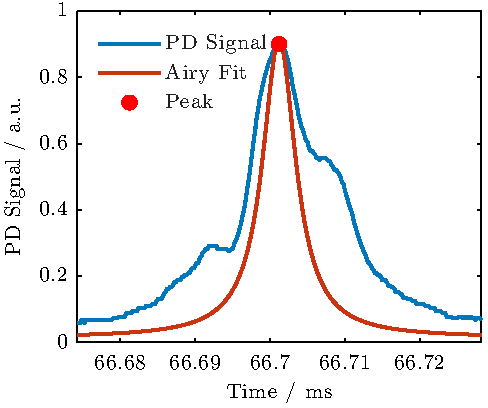
\includegraphics[width=\textwidth]{twoPiezo/Figure_31.pdf}
        \caption{Zoomed-in view of Peak 1.}
        \label{fig:peak1_low}
    \end{subfigure}
    \hfill
    \begin{subfigure}[t]{0.48\textwidth}
        \centering
        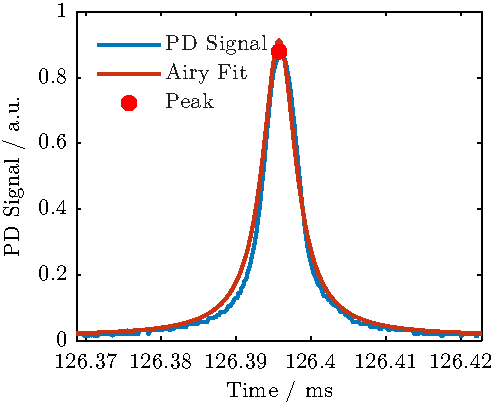
\includegraphics[width=\textwidth]{twoPiezo/Figure_41.pdf}
        \caption{Zoomed-in view of Peak 2.}
        \label{fig:peak2_low}
    \end{subfigure}
    \caption{Zoomed-in views of the detected large peaks of one scan. The left one is cleary still fuzzy and spread out.}
\end{figure}

Once again, this data corresponds to a finesse of $\mathcal{F}\approx11\,000$.
